%===========================================================================
\documentclass[uebung]{ETHIDSCprogramming_dpoc}

%\usepackage{german}
%\usepackage[latin1]{inputenc}
%\usepackage{float}
%\usepackage{amsfonts}
%\usepackage{amssymb}
\usepackage{array, longtable}




%---------------------------------------------------------------------------
 \vorlesungstitel{Dynamic Programming and Optimal Control}
 \vorlesungsnummer{151-0563-01}
 \semester{Fall 2011}
 \info{Contact: Mohanarajah Gajamohan ({\tt gajan@ethz.ch})}

 \uebungsnummer{2}
 \thema{Policy/Value Iteration and Linear Programming}

 \ausgabe{Nov 23, 2011}
 %\vorbesprechung{29.\,10.\,03}
 \abgabe{Dec 07, 2011}
 %\nachbesprechung{Nov 5/19, 2008}

 \textbook{BERTSEKAS}

%---------------------------------------------------------------------------

% Some definitions
\newcommand{\field}[1]{\mathbb{#1}}
\newcommand{\R}{\field{R}}

%---------------------------------------------------------------------------

\sloppy
\begin{document}

\maketitle

\begin{center}
\vspace{0.6cm}
\large\textbf{Policy Iteration, Value Iteration and Linear Programming}
\end{center}
\medskip

Consider the task of driving an under-powered vehicle up a steep mountain road as shown below. Assume that the vehicle remains on the road at all times.
\begin{figure}[h!]
\begin{center}
    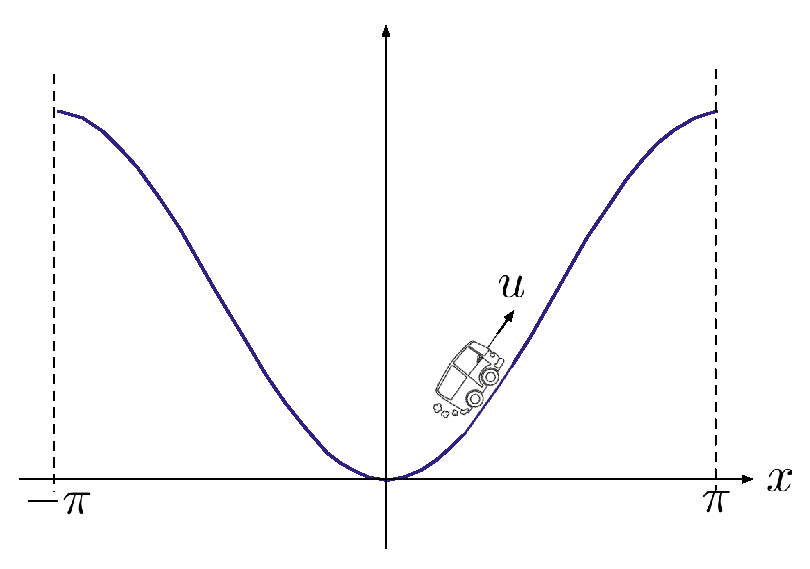
\includegraphics[scale=0.6]{img/mceps.eps}
\end{center}
\end{figure}

There are three possible actions $u$: full throttle forward ($u=u_{\mathrm{max}}, \ u_{\mathrm{max}} > 0$), full throttle backwards ($u=-u_{\mathrm{max}}$) and zero throttle ($u=0$). The discrete time dynamics of the vehicle are given by
\begin{eqnarray}
v_{k+1} &=& v_k + a(v_k,p_k,u_k) \Delta t,  \nonumber \\
p_{k+1} &=& p_k + v_k  \Delta t + 0.5 a(v_k,p_k,u_k) {\Delta t}^2,  \nonumber
\end{eqnarray}
where $v_k$, $p_k$ are the velocity and position of the vehicle along the horizontal direction at the $k^\mathrm{th}$ time instance, $\Delta t$ is the discrete time interval, $a$ is the acceleration along the horizontal direction given by
\begin{equation}
a(v_k,p_k,u_k) = -\frac{\sin p_k \cos p_k}{1+\sin^2 p_k} {v_k}^2 -  \frac{\sin p_k}{1+\sin^2 p_k} g +\frac{1}{(1+\sin^2 p_k)^\frac{3}{2}} u_k \nonumber, 
\end{equation}
and $g$ is the gravitational acceleration equal to $9.81\ \mathrm{ms}^{-2}$. 

The goal is to find the optimal policy that takes the vehicle to the mountain top, $p~=~\pi $ or  $p~=~-\pi $, starting from any given state $[v_0,p_0]$,  $p_0 \in (-\pi,\pi),\ v_0 \in (-v_\mathrm{max},v_\mathrm{max})$, $v_\mathrm{max}~=~6.5~\mathrm{ms}^{-1}$ in minimal time (time optimal policy). 
Discretize the state space and solve the problem in three different ways using the following algorithms:

%\footnote{For testing use $g=9.81$, $u_\mathrm{max} = 1$, $\Delta t = 0.1$ and discretize the state space $[v,x]^\mathrm{T}$,  $v \in (-v_\mathrm{max},v_\mathrm{max}), \ x \in (-\pi,\pi)$ in to a $50 \times 50 $ grid.}

\begin{itemize}
	\item[(i)] Policy Iteration
	\item[(ii)] Value Iteration
	\item[(iii)] Linear Programming
\end{itemize}

\subsubsection*{Deliverables}
Please hand in by e-mail:
\begin{itemize}
\item Your implementation of the above three algorithms along with the following function implementation \footnote{Strictly follow the structure. Grading of this part is automated.}:
 
{\tt [T,Xstar,Ustar,TE] = progEx2Solver(x0, u\_max, dT, gridSize, opt)} 

\textbf{Inputs}

\subitem {\tt x0}: initial state $[v_0, p_0]$, column vector of size $2$ where $v_0 \in (-v_\mathrm{max},v_\mathrm{max})$, $p_0~\in~(-\pi,\pi)$
\subitem {\tt u\_max}: absolute value of the allowed acceleration (throttle) where {\tt u\_max} $\ \in (1,3)$ 
\subitem {\tt dT}: sampling time where {\tt dT} $\ \in [0.1,0.3]$
\subitem {\tt gridSize}: $[\ \mathrm{number\ of\ discretizations\ of\ the\ velocity\ space}\ [-v_\mathrm{max},v_\mathrm{max}]$, $\mathrm{number\ \ of\ discretizations\ of\ the\ position\ space}\ [-\pi,\pi]]$, column vector of size $2$ where each element can take an integer value between $50$ and $70$
\subitem {\tt opt}: algorithm option ({\tt 'P', 'V', 'L'}), type {\tt char}, {\tt 'P'}-Policy Iteration, {\tt 'V'}-Value Iteration, and {\tt 'L'}-Linear Programming

\textbf{Outputs}
\subitem {\tt T}: column vector of time points
\subitem {\tt Xstar}: optimal-state array. Each row in {\tt Xstar} corresponds to the state at a time returned in the corresponding row of T
\subitem {\tt Ustar}: optimal-input array. Each row in {\tt Ustar} corresponds to the state at a time returned in the corresponding row of T
\subitem{\tt TE}: time at which the vehicle reaches the top $p\ =\ \pi $ or  $p\ =\ -\pi $
\item Plot of the cost-to-go values against the discretized  states $[v, p]$: $v \in (-v_\mathrm{max},v_\mathrm{max}),\ p \in (-\pi,\pi)$. You can use the matlab function {\tt surf} to plot.
\item In a PDF file, give the physical interpretation of the
\begin{enumerate}
\item Optimal policy you found 
\item Steep areas in the cost-to-go/state plot.
\end{enumerate}
\end{itemize}
Please include all files into one {\tt zip}-file, which you name {\tt DPOCEx2\_Names.zip}, where {\it Names} 
is a list of the surnames with the initial letter of the first name of all students who have worked
on the solution.\footnote{Up to three students are allowed to work together on the problem.  They will all receive the same grade.} 
Example:  {\tt DPOCEx2\_HuebelN\_GajamohanM.zip}.

Send your file to Gajan ({\tt gajan@ethz.ch}) until the due date indicated in the front page header.  We will send a confirmation upon receiving your e-mail.  You are ultimately responsible that we receive your solution in time.


\subsubsection*{Plagiarism}
When handing in any piece of work, the student (or, in case of a group work, each individual student) listed as author confirms that the work is original, has been done by the author(s) independently and that s/he has read and understood the \textit{ETH Citation etiquette} (http://www.ethz.ch/students/exams/plagiarism\_s\_en.pdf). Each work submitted will be tested for plagiarism.

\end{document}
%===========================================================================
